\documentclass{article}
\author{Grunda}

% Підключення додаткових пакетів
\usepackage[utf8]{inputenc}
\usepackage[ukrainian]{babel}  
\usepackage{amsmath}  
\usepackage{graphicx} 
\usepackage{geometry}  
\usepackage{color}
\usepackage{float}
\usepackage{listingsutf8} % Для відображення коду
\usepackage{caption}    % для підписів до фігур/таблиць
\usepackage{hyperref}   % для гіперпосилань
\usepackage{tikz}
\usetikzlibrary{arrows.meta}
\geometry{left=2.5cm, right=2.5cm, top=2.5cm, bottom=2.5cm}

% Оформлення для коду Python
\lstset{
    language=Python,
    basicstyle=\ttfamily\footnotesize,
    keywordstyle=\color{blue},
    stringstyle=\color{red},
    commentstyle=\color{green},
    numbers=left,
    numberstyle=\tiny\color{gray},
    stepnumber=1,
    numbersep=10pt,
    showstringspaces=false,
    breaklines=true,
    frame=single,
    captionpos=b
}

% Титульна сторінка
\title{Звіт до лабораторної роботи}
\author{Ярослав Грунда \\ Фі-21, ФТІ КПІ}
\date{\today}

\begin{document}

\maketitle 

\tableofcontents  
\newpage

\section{Очищення данних}
Видалення не потрібних данних:
\begin{lstlisting}[language=Python]
df = pd.read_csv("D:/University/third_course/MTAD/lab1/Spotify_Youtube.csv")
df = df.drop(columns=["Unnamed: 0", "Url_spotify", "Uri", "Url_youtube"])
df = df.dropna()
\end{lstlisting}

Видалення викидів:
Видаляємо 1 процент викидів від найбільших і найменших значень кожного числового стовпчика
\begin{lstlisting}[language=Python]
for column in numeric_df.columns:
    lower_bound = numeric_df[column].quantile(0.01)  
    upper_bound = numeric_df[column].quantile(0.99)  
    
    initial_count = df_cleaned.shape[0]
    df_cleaned = df_cleaned[(df_cleaned[column] >= lower_bound) & (df_cleaned[column] <= upper_bound)]
    final_count = df_cleaned.shape[0]
    
    print(f"Column '{column}': removed {initial_count - final_count} rows.")
df_cleaned.reset_index()
print(f"Number of rows before removal: {df.shape[0]}")
print(f"Number of rows after removal: {df_cleaned.shape[0]}")
\end{lstlisting}
Результат:\\
\begin{tabular}{|l|c|}
    \hline
    \textbf{Стовпець} & \textbf{Кількість видалених рядків} \\
    \hline
    Danceability & 376 \\
    Energy & 321 \\
    Key & 0 \\
    Loudness & 203 \\
    Speechiness & 359 \\
    Acousticness & 230 \\
    Instrumentalness & 69 \\
    Liveness & 341 \\
    Valence & 192 \\
    Tempo & 266 \\
    Duration\_ms & 243 \\
    Views & 291 \\
    Likes & 75 \\
    Comments & 50 \\
    Stream & 177 \\
    \hline
    \end{tabular}
    \\
    Кількість рядків до видалення: 19170 \\
    Кількість рядків після видалення: 15977


\section{Статистичні значення}
Функція для обчислення середнього
\begin{lstlisting}[language=Python]
def mean(column):
    return sum(column) / len(column)
\end{lstlisting}
Функція для обчислення усіченого середнього
\begin{lstlisting}[language=Python]
def trimmed_mean(column, trim_percent):
    sorted_col = sorted(column)
    trim_count = int(len(sorted_col) * trim_percent)
    trimmed_col = sorted_col[trim_count:-trim_count]
    return sum(trimmed_col) / len(trimmed_col)
\end{lstlisting}
Функція для обчислення медіани
\begin{lstlisting}[language=Python]
def median(column):
    sorted_col = sorted(column)
    n = len(sorted_col)
    mid = n // 2
    if n % 2 == 0:
        return (sorted_col[mid - 1] + sorted_col[mid]) / 2
    else:
        return sorted_col[mid]
\end{lstlisting}
Функція для обчислення дисперсії
\begin{lstlisting}[language=Python]
def variance(column):
    column_mean = mean(column)
    return sum((x - column_mean) ** 2 for x in column) / (len(column) - 1)
\end{lstlisting}
Функція для обчислення стандартного відхилення
\begin{lstlisting}[language=Python]
def std_dev(column):
    return variance(column) ** 0.5
\end{lstlisting}
Функція для обчислення середнього відхилення
\begin{lstlisting}[language=Python]
def mean_absolute_deviation(column):
    column_mean = mean(column)
    return sum(abs(x - column_mean) for x in column) / len(column)
\end{lstlisting}
Функція для обчислення абсолютного медіанного відхилення
\begin{lstlisting}[language=Python]
def median_absolute_deviation(column):
    col_median = median(column)
    deviations = [abs(x - col_median) for x in column]
    return median(deviations)
\end{lstlisting}
Функція для обчислення всіх показників для обраних стовпців
\begin{lstlisting}[language=Python]
def calculate_statistics(df, columns = None, trim_percent=0.1):
    if isinstance(columns, str):
        columns = [columns]
    elif columns is None:
        columns = df.columns

    results = {}
    for column in columns:
        col_data = df[column].dropna().tolist() 
        stats = {
            'mean': mean(col_data),
            'trimmed_mean': trimmed_mean(col_data, trim_percent),
            'median': median(col_data),
            'variance': variance(col_data),
            'std_dev': std_dev(col_data),
            'mean_absolute_deviation': mean_absolute_deviation(col_data),
            'median_absolute_deviation': median_absolute_deviation(col_data)
        }
        results[column] = stats
    results_df = pd.DataFrame(results).T
    return results_df
\end{lstlisting}
\begin{figure}
    \centering
    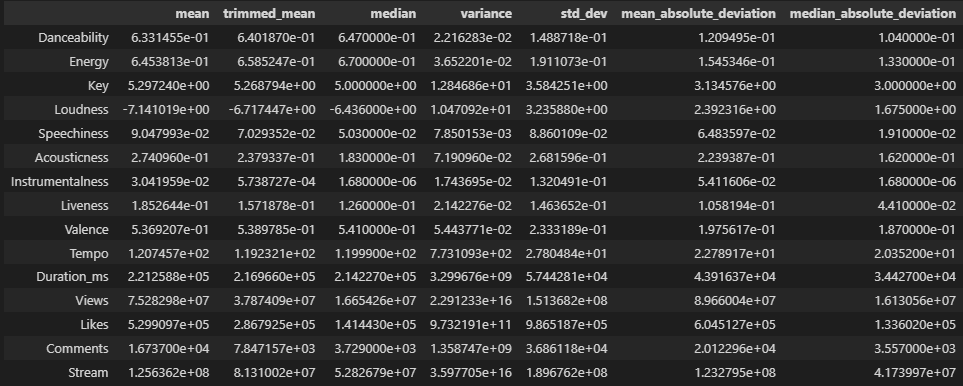
\includegraphics[width=0.8\textwidth]{img/statisticalNumbers.png} % Adjust width as needed
    \caption{Статистичні значення} % Caption for the image
    \label{fig:statistical_numbers} % Label for referencing the figure
\end{figure}
\newpage
\section{Нормалізація}
Нормалізація методом мінімум-максимум
\begin{lstlisting}[language=Python]
def min_max_normalization(df):
    normalized_df = df.copy()
    for column in normalized_df.columns:
        min_val = normalized_df[column].min()
        max_val = normalized_df[column].max()
        normalized_df[column] = (normalized_df[column] - min_val) / (max_val - min_val)
    return normalized_df
\end{lstlisting}
\begin{figure}[ht]
    \centering
    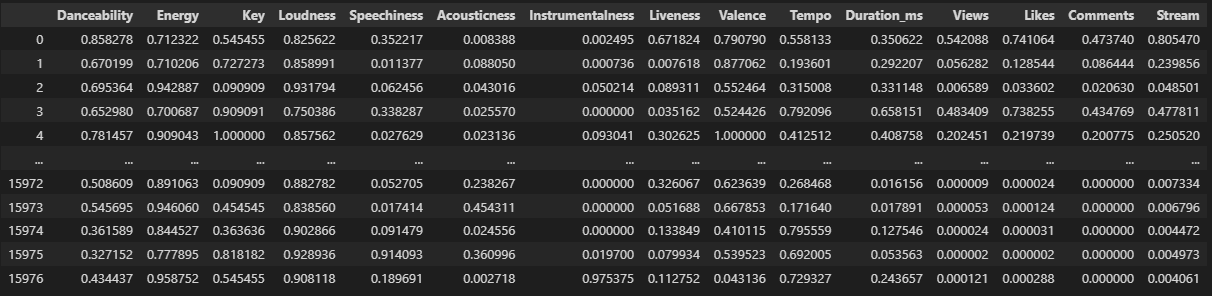
\includegraphics[width=0.8\textwidth]{img/minmax.png} % Adjust width as needed
    \caption{MinMax нормалізація} % Caption for the image
    \label{fig:minmax} % Label for referencing the figure
\end{figure}
\newpage
Нормалізація методом середньої нормалізації
\begin{lstlisting}[language=Python]
def mean_normalization(df):
    normalized_df = df.copy()
    for column in normalized_df.columns:
        mean_val = normalized_df[column].mean()
        std_dev = normalized_df[column].std()
        normalized_df[column] = (normalized_df[column] - mean_val) / std_dev
    return normalized_df
\end{lstlisting}

\begin{figure}
    \centering
    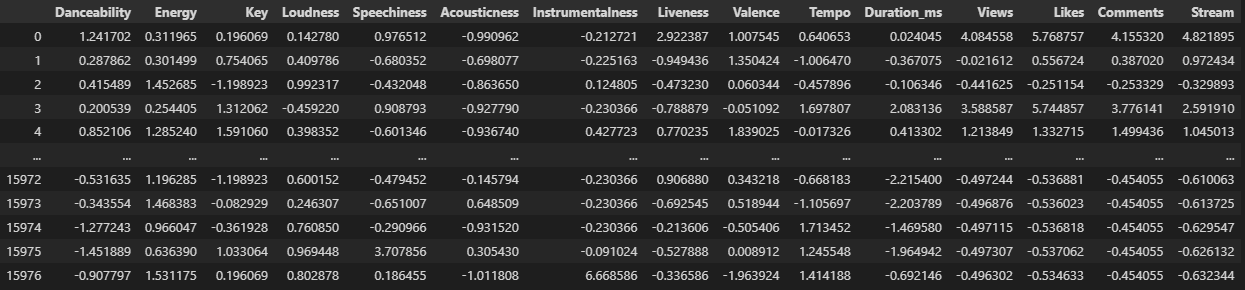
\includegraphics[width=0.8\textwidth]{img/meannorm.png} % Adjust width as needed
    \caption{Середня нормалізація} % Caption for the image
    \label{fig:meannorm} % Label for referencing the figure
\end{figure}

\section{Графіки}

\begin{figure}[ht]
    \centering
    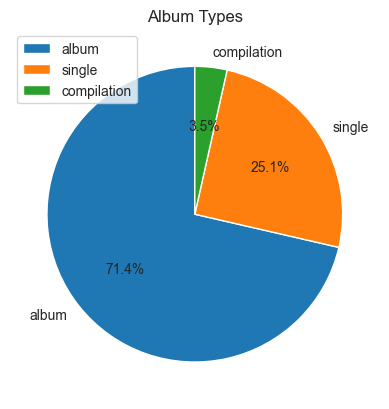
\includegraphics[width=0.7\textwidth]{img/albumtypes.png} % Adjust width as needed
    \caption{} % Caption for the image
\end{figure}
\begin{figure}[ht]
    \centering
    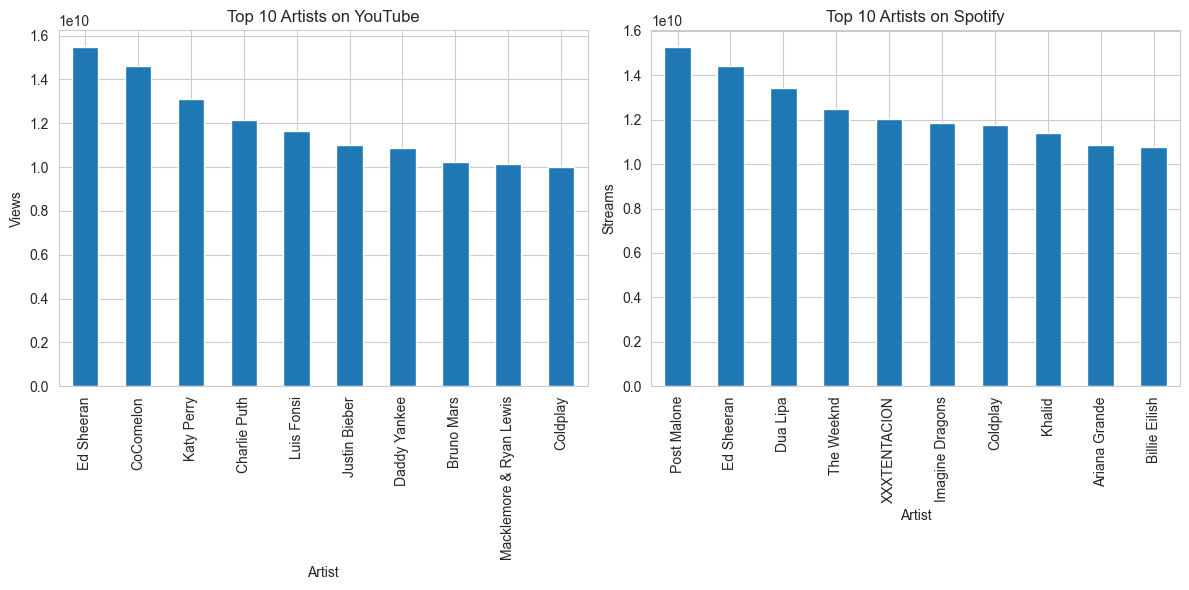
\includegraphics[width=0.8\textwidth]{img/top10artists.png} % Adjust width as needed
    \caption{} % Caption for the image
\end{figure}
\begin{figure}[ht]
    \centering
    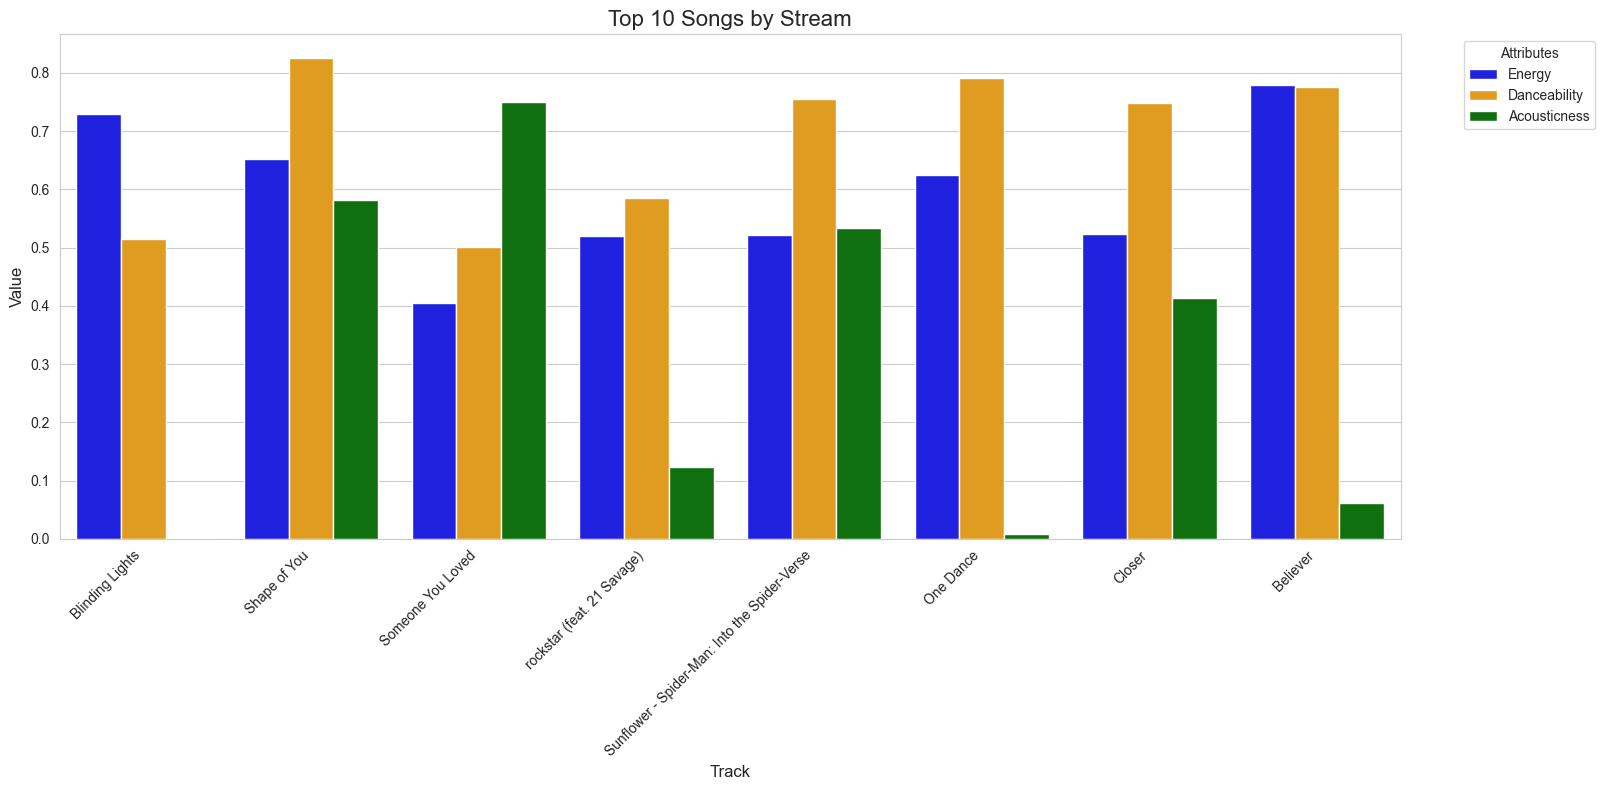
\includegraphics[width=0.8\textwidth]{img/topsongs.png} % Adjust width as needed
    \caption{} % Caption for the image
\end{figure}
\end{document}
